\chapter{Software-Architekturen für mobile Robotersysteme}
\section{Probleme und Anforderungen}
\subsection{Definition mobile Roboter}
\enquote{Unter einem Roboter verstehen wir eine frei programmierbare Maschine, die auf Basis von Umgebungssensordaten in geschlossener Regelung in Umgebungen agiert, die zur Zeit der Programmierung nicht genau bekannt und/oder dynamisch und oder nicht vollständig erfassbar sind.}
$\Rightarrow$ \textbf{Joachim Herzberg, Mobile Roboter}
\subsection{Umgebung mobiler Roboter}
Bei \textbf{mobilen Robtoern} ist die Umgebung im Detail \textbf{nicht bekannt und generell nicht kontrollierbar}
\begin{itemize}
	\item Alle Aktionen sind von der aktuellen Umgebung abhängig
	\item Details sind erst zum Zeitpunkt der Ausführung der Aktionen bekannt
	\item Mobile Roboter müssen in einer geschlossenen Regelung
		\subitem die Umgebung mit Sensoren erfassen
		\subitem die Daten auswerten
		\subitem Aktionen daraus planen
		\subitem Aktionen mittels Koordination der Aktuatoren umsetzen
\end{itemize}
\subsection{Roboterkontroll-Architekturen}
\paragraph{Herausforderungen}
\begin{itemize}
	\item Robotersystem besteht aus den Gebieten \textbf{Wahrnehmung}, \textbf{Planung} und \textbf{Handlung}
	\item Herausforderungen an eine Roboterkontroll-Architektur, sie muss:
	\subitem Sensorwerte erfassen und auswerten
	\subitem Pfade planen
	\subitem Hindernisse vermeiden
	\subitem Komplexe Algorithmen in langen Zeitzyklen ausführen
\end{itemize}
\paragraph{Probleme bei der Software-Erstellung zur Roboterkontrolle}
\begin{itemize}
	\item Roboter sind eingebettete Systeme, die in geschlossener Regelung laufen und die Sensorströme in \textbf{Echtzeit verarbeiten} müssen
	\item Untschiedliche Aufgaben --> Unterschiedliche Zeitzyklen
	\item Unterschiedlicher Zeitskalen --> kein standardisierter Kontroll- oder Datenfluss den die Architektur abbilden könnten
	\item Für etliche algorithmische Teilprobleme sind \textbf{keine effizienten Verfahren} bekannt
	\item \textbf{Prozessorkapazität ist begrenzt}
\end{itemize}
\subsection{Anforderungen an das Kontrollsystem eines autonomen Roboters}
\paragraph{Robustheit}
\begin{itemize}
	\item Die Umgebung des Systems kann sich ständig ändern
	\item Auf eine Umgebungsänderung sollte der Roboter sinnvoll reagieren und nicht verwirrt stehen bleiben.
	\item Verwendete Modelle der Umgebung sind ungenau.
\end{itemize}
\paragraph{Unterschiedliche Ziele}
\begin{itemize}
	\item Der Roboter verfolgt zu einem Zeitpunkt eventuell Ziele, die im Konflikt zueinander stehen.
	\item \textbf{Beispiel}: der Roboter soll ein bestimmtes Ziel ansteuern, dabei aber Hindernissen ausweichen.
\end{itemize}
\paragraph{Sensorwerte von mehreren Sensoren}
\begin{itemize}
	\item Sensordaten könen verrauscht sein
	\item Sensoren können fehlerhafte oder inkonsistente Messwerte liefern, weil der Sensor z.B. außerhalb seines Bereichs misst für den er zuständig ist und dies nicht überprüfen kann.
\end{itemize}
\paragraph{Erweiterbarkeit}
\begin{itemize}
	\item Wenn der Roboter neue Sensoren erhält, sollte dies leicht in das Programm integriert werden können.
\end{itemize}
\section{Mögliche Modelle}
\subsection{Klassisches Modell - der funktionale Ansatz}
Das \textbf{klassische Model} wird auch als hierarchisches Model oder funktionales Model bezeichnet.
Ist ein Top-Down Ansatz, besteht aus drei Abstraktionsebenen
\begin{itemize}
	\item Die unterste Ebene: \textbf{Pilot}
	\item Mittlere Eben: \textbf{Navigator}
	\item Oberste Ebene: \textbf{Planer}
\end{itemize}
\textbf{Sense-Think-Act-Cycle} oder \textbf{SMPA} (Sense - Model - Plan - Act).
\begin{itemize}
	\item Sensordaten, die vom Fahrzeut geliefert werden, werden in den zwei unteren Ebenen vorverarbeitet.
	\item Konstruktion oder Aktualisierung eines Weltmodells
	\item \textbf{Planer} ist die Basis aller Entscheidungen basieren auf dem zugrundelgenden Weltmodell
	\item Tatsächliche Fahrbefehle werden durch unterste Ebene ausgeführt
\end{itemize}
Zyklus wird ständig wiederholt $\Rightarrow$ wenn alle Ebenen richtig funktionieren resultiert daraus ein intelligentes Verhalten und die Erfüllung der Aufgabe.
\paragraph{Nachteile}
\begin{itemize}
	\item \textbf{Sequentieller Ansatz}, \textbf{lange Kontrollzykluszeit}
	\item Gesamtsystem anfällig, $\Rightarrow$ fällt ein Modul scheitert das Gesamtsystem
	\item Die Repräsentation der Umgebung muss alle notwendigen Informationen enthalten, damit ein Plan entwickelt werden kann.
	Planer hat nur Zugriff auf das Weltmodell $\Rightarrow$ während Planer aktionen ausarbeitet, könnte sich die Umwelt schon wieder geändert haben.
\end{itemize}
\subsection{Verhaltensbasiertes Modell}
\paragraph{Grundlegender Gedanke} Intelligentes Verhalten wwird nicht durch komplexe, monolithische Kontrollstrukturen erzeugt, sondern durch das Zusammenführen der richtigen einfachen Verhalten und deren Interaktion.
\paragraph{Definition}
\begin{itemize}
	\item Engere Verbindung zwischen \textbf{Wahrnehmung} und \textbf{Aktion}
	\item Jede \textbf{Roboterfunktionalität} wird in einem \textbf{Behavior} gekapselt
	\item Alle \textbf{Behaviors} werden \textbf{parallel ausgeführt}
	\item Jedes Behavior Modul operiert unabhängig von den anderen
	\item Alle Behaviors können auf alle Fahrzeugsensoren zugreifen und gewissermaßen die Aktuatoren ansteuern.
\end{itemize}
\paragraph{Beispiel}
\textbf{Subsumption Architektur nach Brooks}
\newpage
\subsection{Hybrider Ansatz}
\begin{itemize}
	\item Nutzt die Vorteile der \textbf{Subsumption Architektur} und der \textbf{SMPA-Architektur}
	\item Der verhaltensbasierte Anteil ist nicht geeignet, auf längere Sicht zielgerichtet Aktionen zu koordinieren $\Rightarrow$ SMPA-Anteil
\end{itemize}
\begin{figure}[H]
	\begin{center}
		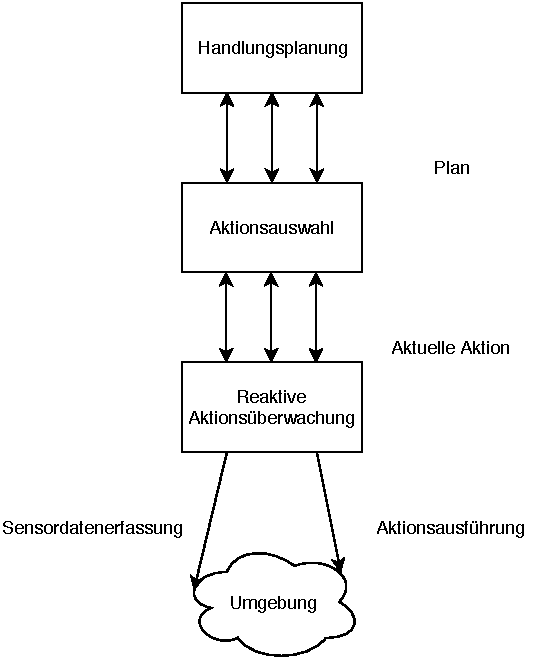
\includegraphics[scale=0.9]{Resources/PDF/HybridModel}
		\caption{Schema der Hybridmodell Schichten}
		\label{fig:PDF/HybridModel}
	\end{center}
\end{figure}
\begin{itemize}
	\item Die \textbf{Handlungsplanung} arbeitet auf hoher, strategischer Stufe in langen Zeitzyklen
	\item Die \textbf{reaktive Aktionsüberwachung} enthält die Verhaltensbausteine auf operativer Ebene, die in schellen Zeitzyklen die physische Roboteraktion anstoßen und überwachen
	\item die \textbf{mittlere Kontrollebene} hat die taktische Aufgabe, die jeweils \textbf{nächste Aktion aus dem Plan auszusuchen} zu instanzieren und auf die Ebene der Verhaltensbausteine zu zerlegen
	Des weiteren muss die die Rückmeldung von der Aktionsüberwachung interpretieren und entscheiden ob eine Aktion erfolgreich abgeschlossen ist. $\Rightarrow$ entscheiden ob die Handlungsplanung einen anderen Plan erstellen muss
\end{itemize}
\newpage
\paragraph{Kritik}
\begin{itemize}
	\item Mittlere Komponente benötigt den größten konzeptuellen und programmiertechnischen Aufwand
	\item Das mittlere Teilproblem ist deutlich komplexer als die beiden anderen
\end{itemize}
\subsection{Probabilistische Robotik}
\begin{itemize}
	\item Probabilistische Robotik berücksichtigt die \textbf{Unsicherheit der Wahrnehmund und der Aktionen}
	\item \textbf{Schlüsselidee} Information in Form von Wahrscheinlichkeitsdichten repräsentieren
	\item Eine Lokalisierung der Roboter wird unter Verwendung von wahrscheinlichkeitstheorie oder einer Wahrscheinlichkeitsverteilung eine Aussage über die Umgebung treffen
	\item \textbf{Probabilistische Wahrnehmung}: wenn man Sensorwerte schätzen kann, dann kann man mit Wahrscheinlichkeitstheorie/Wahscheinlichkeitsverteilung eine Aussage über die Umgebung treffen
	\item \textbf{Probabilistisches Handeln}: aufgrund der Unsicherheit über die Umgebung ist auch das Handeln mit Unsicherheit behaftet.
	Mit probabilistischen Ansätzen besteht die Möglichkeit Entscheidungen trotz Unsicherheit zu treffen
\end{itemize}
\paragraph{Vorteil} probabilistische Verfahren können auch mit weniger präzisen Umgebungsmodellen angewandt werden.
\paragraph{Nachteil} weniger effizient wegen komplexer Berechnungen, Approximation erforderlich
\subsection{Subsumption-Architektur in Bezug auf die Anforderungen des Robotersteuerungssystems}
\paragraph{Robustheit}
\begin{itemize}
	\item Wenn einige Steuerungsmodule ausfallen, arbeiten bei der Subsumption-Architektur in die restlichen Schichten einwandfrei $\Rightarrow$ \textbf{eingeschränktes, aber sinnvolles Verhalten möglich}
\end{itemize}
\paragraph{Unterschiedliche Ziele}
\begin{itemize}
	\item Mehrere Teilsituation können verschiedene Verhaltenselemente sinvoll machen, die sich widersprechen können.
	\item Die Wichtigkeit einer Handlung hängt vom Kontext ab, d.h. höhere Ziele können niederere Ziele ersetzen.
	\item Alle zu einem Zeitpunkt möglichen Verhaltenselemente werden parallel bearbeitet.
	\item Das \textbf{resultierende Verhalten wird in Abhängigkeit von Umwelteinflüssen dynamisch} bestimmt
	\item Das Gesamtergebnis hängt nicht von einer übergeordneten Instanz ab
\end{itemize}
\paragraph{Sensorwerte von mehreren Sensoren}
\begin{itemize}
	\item Der Roboter muss auch bei inkonsistenten Informationen eine Entscheidung fällen
	\item Die Subsumption-Architektur sieht keine zentrale Verarbeitung und Speichung der Umweltdaten
	\item Jedes Modul reagiert nur auf die Daten einzelner Sensoren, es muss \textbf{kein konsistentes Abbild der Umwelt erschaffen werden}
\end{itemize}
\paragraph{Erweiterbarkeit}
Das bestehende Verhalten kann jederzeit durch Hinzufügen weiterer Schichten um komplexere Funktionen erweitert werden
\section{ROS - Robot Operating System}
\subsection{Entwicklung}
\begin{itemize}
	\item \textbf{Das Architekturschema für Roboterkontrollsoftware} gibt es nicht $\Rightarrow$ deshalb heute auch Unterstützung der Roboter-Softwareentwicklung durch Middleware wie ROS
	\item \textbf{Zweck}: soll die Entwicklung von Software für Roboter vereinfachen und wiederkehrende Aufgaben standardisieren
	\item Standard für Robotoerkontrollsoftware
\end{itemize}
\subsection{Design Prinzipien}
\begin{figure}[H]
	\begin{center}
		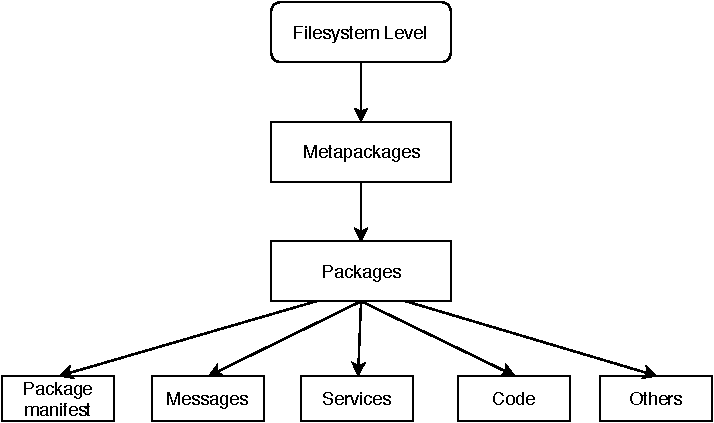
\includegraphics[]{Resources/PDF/FileSystem}
		\caption{Filesystem, das ROS zugrunde liegt}
		\label{fig:PDF/FileSystem}
	\end{center}
\end{figure}
\begin{itemize}
	\item Ein Package beinhaltet die ROS Prozesse, welche auch Nodes genannt werden
	\item Komplexe Prozesse werden durch Netzwerke von Nodes bewerkstelligt
	\item Roboterkontrollprogramm besteht aus vielen Prozessen, die potentiell über mehrere Rechner verteilt sein können
	\item Wichtigster Knoten ist der Master $\Rightarrow$ Abwicklung der internen Kommunikation
	\item Andere Knoten können nur starten, wenn ein Master existiert
	\item Nodes müssen sich beim Master anmelden
	\item Funktionalität (Kommandods, Ausführung v. Algorithemen) wird in eigenen Nodes realisiert
	\item Nodes sind in verschiedene Prozesse getrennt $\Rightarrow$ fehlerhafte Knoten hat i.d. Regel wenig Auswirkungen auf die anderen
	\item Knoten werden über Publish-Subscribe verknüpft
	\item \textbf{Asynchrone Nachrichten} werden durch Topics ausgetauscht
	\item \textbf{Synchrone Nachrichten} werden durch Services ausgetauscht
\end{itemize}
\subsection{Publish - Subscribe}
\paragraph{Nodes} sind Software-Module, die die Verarbeitung durchführen. Sie kommunizieren über Topics miteinander und tauschen dabei Nachrichten.
\paragraph{Kommunikation}
Die Kommunikation basiert auf einem \textbf{Publish Subscribe Pattern}
\begin{itemize}
	\item Wenn Daten weitergegeben werden sollen, wird ein Publisher erzeugt
	\item Publisher registriert sich beim Master und gibt Topics an
	\item Daten können in anderen Knoten abgerufen werden -- dazu wird ein (oder mehrere) Subscriber angelegt
	\item Subscriber frägt beim Master bezüglich gewünschten Topics an
	\item Daten werden über TCP/IP Sockets übertragen
\end{itemize}
\paragraph{Topics}
\begin{itemize}
	\item Themen, zu denen die Nodes Messages versenden
	\item Topics sind einfach Strings
	\item Verschiedene Nodes können zu einem bestimmten Topic Nachrichten versenden
	\item Ein Node kann sich prinzipiell zu mehreren Topics einschreiben und mehrere Topics publizieren
\end{itemize}
\paragraph{Services}
\begin{itemize}
	\item Nachteil von Publish Subscribe wird durch Services geschlossen
	\item Sind eine weitere Art, wie Nodes kommunizieren können
	\item Synchroner Nachrichtenaustausch mithilfe von Requests, welche von anderen Nodes mit einer Response beantwortet werden
	\item Ein Knoten registriert eine Aktion (Service), namentlich beim Master
	\item Ein Service Caller kann die Ausführung eines Services anstoßen, sobald dieser verfügbar ist
	\item geeignet für RMI oder einmalige Anfragen
\end{itemize}
\paragraph{Messages}
\begin{itemize}
	\item werden von Nodes bei der Kommunikation
	\item Messages sind streng typisierte, möglicherweise verschachtelte Datenstrukturen, die aus den primitiven Typen int, float, bool bestehen
	\item Eine Message kann andere Messages oder Felder von Messages enthalten
\end{itemize}
\subsection{Parameter Server und Konfigurationsdateien}
\begin{itemize}
	\item Der ParameterServer auf dem Master Knoten enthält eine Art Wörterbuch für Werte.
	\item Alle Ressourcen wie Knoten, Nachrichten oder Parameter existieren in einer hierarchischen Namensstruktur.
	\item Speichert z.B. Konfigurationsdateien
\end{itemize}



%seite 25 kapitel 2